
\chapter{Neural Networks}

In this chapter, we'll briefly discuss some concepts on \textit{Neural Networks} (or NNs) and a little bit of \textit{Machine Learning}. NNs will later be used as a function approximator in the Policy Gradient chapter and was also a subject of study during the making of this work.

\section{Machine Learning}
Nowadays, as the Internet continues to expand, we have more and more information available and stored everyday. Due to that large volume of data, analyzing it and extracting meaningful information has become a task increasingly difficult for humans to perform. From that challenge, the concept of \textit{Machine Learning} arises.

Machine learning can be defined as a set of techniques (or algorithms) that allows for a computer program to extract information, identify paterns and relationships in large amounts of data, in such a way a human cannot.

According to \cite{Mitchell}, \textit{"A computer program is said to learn from experience $E$ with respect to some class of tasks $T$ and performance measure $P$ if its performance at tasks in $T$, as measured by $P$, improves with experience $E$"}.

\cite{Goodfellow-et-al-2016} broke machine learning down to 3 main paradigms:
\begin{itemize}
    \item In \textbf{Supervised Learning}, we have a dataset containing features, but each example is also associated with a \textit{label} or \textit{target}. For example, a dataset containing emails labeled as \textbf{spam} or \textbf{not spam}. A supervised learning algorithm can study this dataset and learn to classify whether an email is a spam or not.
    \item In \textbf{Unsupervised Learning}, we have a dataset containing many features, but no labels. Then, the goal is to learn useful properties of the structure of this dataset. In the context of deep learning, we usually want to learn the entire probability distribution that generated the dataset. Some other unsupervised learning algorithms perform other roles, like clustering, which consists of dividing the dataset into clusters of similar data.
    \item Then, there's \textbf{Reinforcement Learning}, where we don't have a fixed dataset. Instead, RL algorithms interact with the environment, forming a feedback loop between the learning system and what it has experienced.
\end{itemize}

\section{Neural Networks}
Neural Networks are a set of machine learning algorithms, whose structure is strongly related with the structure of the human brain. 
\begin{figure}[H]
    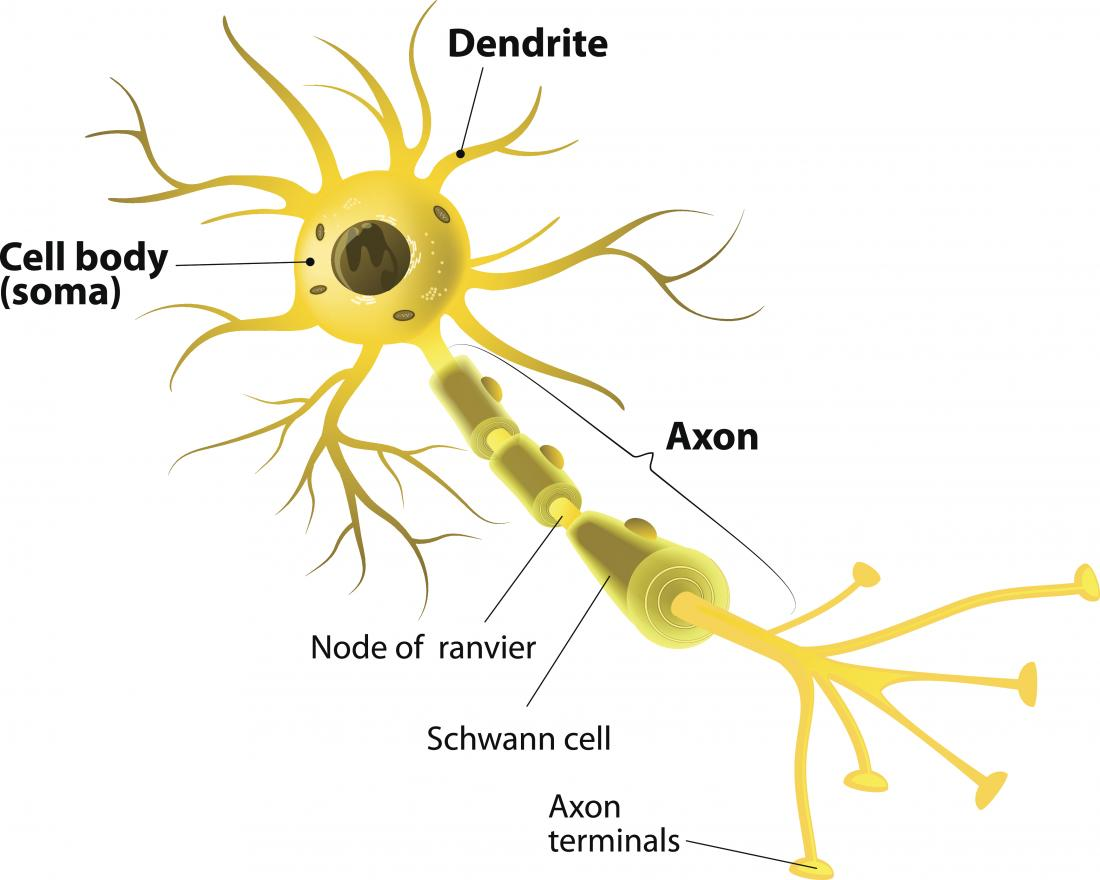
\includegraphics[width=\textwidth]{neuron-diagram}
    \caption{Source: \href{https://www.medicalnewstoday.com/articles/320289}{MedicalNewsToday}}
\end{figure}
The main structural cells responsible for processing information are divided into 3 main parts:
\begin{itemize}
    \item \textbf{Dendrites:} filaments responsible for receiving and transporting stimulus coming from the environment or other cells of the body.
    \item \textbf{Body cell:} processes the information gathered by the dendrites.
    \item \textbf{Axon:} transmits the nervous impulses generated by the cell body to the other cells through the axon terminals.
\end{itemize}
In summary, upon receiving stimuli, the cell body processes those signals and if the result exceeds a certain threshold value, the neuron fires a nerve impulse indicating it reacted to the input signals, which are further transmitted by other neurons to other neurons or cells.

The human brain processes information processes in order $10^{-3}$ seconds, having a network of about 10 billion neurons densely connected, making it a huge, complex and efficient processing powerhouse, performing tasks like recognizing images and audios better than any machine. In an attempt to recreate a system that was able to operate like a human brain, the concept or \textit{Artificial Neural Networks} was idealized.

\cite{haykin2009neural} cites the following useful properties and capabilities:
\begin{itemize}
    \item \textbf{Nonlinearity:} an artificial neuron can be linear or nonlinear. Therefore, a neural network, made up of an interconnection of nonlinear neurons, is itself nonlinear. Nonlinearity is a highly important property, particularly if the underlying physical mechanism responsible for generation of the input signal (e.g., speech signal) is inherently nonlinear.
    \item \textbf{I/O Mapping:} neural networks perform very well in supervised learning tasks, where we have labeled data. Each piece of data is used to update the synaptic bias of the network such that the difference between the expected output and the actual output is minimized.
    \item \textbf{Adaptivity:} neural networks have the capability to adapt their synaptic weights to changes in the surrounding environment. 
    \item \textbf{Evidential Response:} in particular, a neural network trained to operate in a specific environment can be easily retrained to deal with minor changes in the operating environmental conditions.
    \item \textbf{Contextual Information:} in the context of pattern classification, a neural network can be designed to provide information not only about which particular pattern to select, but also about the confidence in the decision made. This latter information may be used to reject ambiguous patterns, should they arise, and thereby improve the classification performance of the network.
    \item \textbf{Uniformity of Analysis and Design:} neural networks enjoy universality as information processors, in a sense that the same notation is used in all domains involving the application of neural networks, making it possible to share techniques and theories between models with different purposes.
    \item \textbf{Neurobiological Analogy:} the design of a neural network is motivated by analogy with the brain, which is a living proof that parallel processing is not only physically possible, but also fast and powerful.
\end{itemize}